\documentclass[output=paper,colorlinks,citecolor=brown]{langscibook}
\author{Tatiana Nikitina\affiliation{LLACAN (CNRS, INALCO)}\orcid{}\lastand Yvonne Treis\affiliation{LLACAN (CNRS, INALCO)}\orcid{}}
\title{The use of manner demonstratives in discourse: A contrastive study of Wan (Mande) and Kambaata (Cushitic)}
\abstract{This chapter compares manner demonstratives in two unrelated African languages, Kambaata (Cushitic, Ethiopia) and Wan (Mande, Côte d’Ivoire). Both languages have specialised manner demonstratives yet differ strikingly in their typological profile and in the way the manner demonstratives behave syntactically. Through systematic comparison of data from both languages, similarities, which are likely due to common semantic mechanisms of meaning extension, and differences, which are likely due to structural differences between the languages, are identified. It is argued that, despite the shared core meanings, manner demonstratives belong to different syntactic classes in Kambaata and in Wan. The difference in syntactic category helps account for the striking dissimilarities in the range of attested extended uses.}
\IfFileExists{../localcommands.tex}{
  % add all extra packages you need to load to this file

\usepackage{tabularx,multicol}
\usepackage{url}
\urlstyle{same}

\usepackage{listings}
\lstset{basicstyle=\ttfamily,tabsize=2,breaklines=true}

\usepackage{tabularx}
\usepackage{langsci-optional}
\usepackage{langsci-lgr}
\usepackage{langsci-gb4e}

\usepackage[linguistics,edges]{forest}

\usepackage{tikz}





  \newcommand*{\orcid}{}

\makeatletter
\let\thetitle\@title
\let\theauthor\@author
\makeatother

\newcommand{\togglepaper}[1][0]{
  \bibliography{../localbibliography}
  \papernote{\scriptsize\normalfont
    \theauthor.
    \thetitle.
    To appear in:
    Change Volume Editor \& in localcommands.tex
    Change volume title in localcommands.tex
    Berlin: Language Science Press. [preliminary page numbering]
  }
  \pagenumbering{roman}
  \setcounter{chapter}{#1}
  \addtocounter{chapter}{-1}
}

\newcommand{\glopa}{\textsc{opa}}
\newcommand{\glme}{\textsc{top}}
\newcommand{\glte}{\textsc{nfin}}
\newcommand{\glta}{\textsc{nfin}}
\providecommand{\citegen}[1]{\citeauthor{#1}'s (\citeyear*{#1})}

% \newcommand{\sectref}[1]{Section~\ref{#1}}
  %% hyphenation points for line breaks
%% Normally, automatic hyphenation in LaTeX is very good
%% If a word is mis-hyphenated, add it to this file
%%
%% add information to TeX file before \begin{document} with:
%% %% hyphenation points for line breaks
%% Normally, automatic hyphenation in LaTeX is very good
%% If a word is mis-hyphenated, add it to this file
%%
%% add information to TeX file before \begin{document} with:
%% %% hyphenation points for line breaks
%% Normally, automatic hyphenation in LaTeX is very good
%% If a word is mis-hyphenated, add it to this file
%%
%% add information to TeX file before \begin{document} with:
%% \include{localhyphenation}
\hyphenation{
affri-ca-te
affri-ca-tes
ana-phor-ic
poly-semy
Spra-chen
Fi-scher
Al-chemist
de-mon-stra-tive
Mül-ler
Brea-ker
Hix-kar-ya-na
Que-chua
Unga-rin-jin
Alam-blak
Wam-bon
da-ta-base
quasi-quo-ta-tions
Pisch-lö-ger
de-mon-stra-tions
Ar-khan-gel-skiy
}
\hyphenation{
affri-ca-te
affri-ca-tes
ana-phor-ic
poly-semy
Spra-chen
Fi-scher
Al-chemist
de-mon-stra-tive
Mül-ler
Brea-ker
Hix-kar-ya-na
Que-chua
Unga-rin-jin
Alam-blak
Wam-bon
da-ta-base
quasi-quo-ta-tions
Pisch-lö-ger
de-mon-stra-tions
Ar-khan-gel-skiy
}
\hyphenation{
affri-ca-te
affri-ca-tes
ana-phor-ic
poly-semy
Spra-chen
Fi-scher
Al-chemist
de-mon-stra-tive
Mül-ler
Brea-ker
Hix-kar-ya-na
Que-chua
Unga-rin-jin
Alam-blak
Wam-bon
da-ta-base
quasi-quo-ta-tions
Pisch-lö-ger
de-mon-stra-tions
Ar-khan-gel-skiy
}
  \togglepaper[1]%%chapternumber
}{}

\begin{document}
\maketitle
\shorttitlerunninghead{The use of manner demonstratives in discourse}

\section{Introduction}\label{sec:nikitina:1}

%Still to be done:
%Repair tables
%keep examples together (no page breaks in examples), I tried \protectedex{…} but this didn't work
%avoid orphans
%repair hyphenations of hyphenated words, they spill into the margins

Manner demonstratives are deictic expressions that identify a way of carrying out an event or the extent to which a property holds, as observed in the speech situation (exophoric use) or expressed in the preceding discourse (endophoric anaphoric use). Manner demonstratives are generally assumed to be adverbs (cf. \citealt{Diessel1999Book}: 74). We take as our starting point a semantic definition of “manner demonstrative” since, as we will see, the syntactic category to which they belong in different languages may vary. Despite a recent increase of interest in manner demonstratives on the part of the typological community (e.g. \citealt{Guérin2015}, \citealt{König2017}, \citealt{KönigUmbach2018}), they remain poorly studied even in well-described languages. The ways they function in discourse, in particular, remain critically underexplored, so that the few existing studies focusing on their grammaticalisation (e.g. \citealt{König2015}) are still dissociated from synchronic corpus-based studies of new and emergent usage.\footnote{Notable exceptions include \citet{KönigNishina2015} on Japanese, \citet{Shor2018} on Hebrew \textit{kaχa}, \citet{KarssenbergLahousse2018} on French \textit{ainsi}, and Keevallik (e.g. \citeyear{Keevallik2005}, \citeyear{Keevallik2010}) on Estonian.}

This study is a contrastive description of the use of manner demonstratives in two unrelated African languages, Kambaata (Cushitic, Ethiopia) and Wan (Mande, Côte d’Ivoire). We chose to compare these two languages, since they both have specialised manner demonstratives yet differ strikingly in their typological profile and in the way the manner demonstratives behave syntactically. Through systematic comparison of data from Kambaata and Wan we hope to identify similarities (which are likely due to common semantic mechanisms of meaning extension) and differences (which are likely due to structural differences between the languages), and to address the challenge of accounting for these similarities and differences within the same model.

We first discuss and classify the common uses attested in both languages (\sectref{sec:nikitina:2}; these uses, we argue, correspond to the “core” meanings of manner demonstratives, which we predict to cluster in other languages as well. We then turn to differences in the ways manner demonstratives behave syntactically in the two languages. We argue that despite their close semantic similarity, manner demonstratives belong to different syntactic classes in Kambaata and in Wan (\sectref{sec:nikitina:3}). The difference in syntactic category helps us account for the striking dissimilarities in the range of attested extended uses. We use a semantic map approach to model the differences, and end with a brief discussion of the study’s methodological and theoretical implications (\sectref{sec:nikitina:4}).


\section{Same core uses}\label{sec:nikitina:2}

\subsection{Contextually salient manner and represented speech}\label{sec:nikitina:2.1}


Manner demonstratives of Kambaata and Wan are characterised by strikingly similar core uses. They occur most frequently in two types of context, indexing either contextually salient manner or instances of represented speech.

Contextually salient manner can be inherent in the current speech situation, as in \REF{ex:nikitina:1a} and \REF{ex:nikitina:1b}, or it may be suggested by an accompanying gesture, as in \REF{ex:nikitina:2a} and \REF{ex:nikitina:2b}. Both uses are deictic: in order to interpret the manner to which the demonstrative refers it is important to observe the situation in which they were uttered. In \REF{ex:nikitina:1a}, the manner demonstrative refers to the way the addressee is acting. In \REF{ex:nikitina:1b}, it indexes the looks of the child present at the site where the sentence is uttered.\footnote{All Wan examples are from a corpus of spontaneous oral data (consisting mostly of narratives). The Kambaata examples are from three different types of source: spontaneous oral data (indicated as: [oral]), local written publications (indicated as: [written]) and from elicitation (indicated as: [elicited]). In the data collection, direct translation elicitation was generally avoided. Instead speakers were asked to come up with near-natural mock dialogues for situations that were laid out by the researcher. Additional elicitations were made on the basis of examples attested in recordings, written text data and mock dialogues.}


\ea\label{ex:nikitina:1} {Manner inherent in the current speech situation}\\
\ea\label{ex:nikitina:1a} {Kambaata [written]}\\
\gll Lankíi harabas-á \textbf{hitt-íta} torr-itókkoont!\\
     again dirt-\textsc{m.acc} like\_this[1]\textsc{{}-f.acc} throw-\textsc{2f.appr}\\
\glt (Speaker sees addressee dropping dirt in the front yard and tells her off:) ‘Don’t throw the dirt away again \textbf{like} \textbf{this}!’
\ex\label{ex:nikitina:1b} {Wan}\\
\gll àà ɓāā n\={ɛ} é kēé wà, ɓāā n\={ɛ} é zièziè yā \textbf{kēé} wà\\
     \textsc{intj} \textsc{log+aln} child \textsc{def} like\_this not \textsc{log+aln} child \textsc{def} ugly with like\_this not\\
\glt ‘Oh, my child is not like this, my child is not ugly \textbf{like} \textbf{this}.’
\z
\z

In \REF{ex:nikitina:2a} and \REF{ex:nikitina:2b}, the relevant manner is represented by a gesture, so that, in order to interpret the manner demonstrative, the listener needs access to the accompanying visual information.

\ea\label{ex:nikitina:2} {Manner suggested by an accompanying gesture}\\
\ea\label{ex:nikitina:2a} {Kambaata [elicited]}\\
\gll \textbf{Hitt-íta} ass-í fann-óomm\\
     like\_this\textsc{[1]-f.acc} do-\textsc{1s.pco} open-\textsc{1s.pfv}\\
\glt (Speaker demonstrates his opening technique:) ‘I opened it \textbf{like} \textbf{this}.’ 
\ex\label{ex:nikitina:2b} {Wan}\\
\gll è é \={ɔ} wō \textbf{kēé}\\
     \textsc{3sg} \textsc{refl} hand did like\_this\\
\glt ‘He made a gesture with his hand \textbf{like} \textbf{this}.’
\z
\z

In addition to pointing to a contextually salient manner, the same markers can also be used to refer to a following instance of reported speech. Unlike in \REF{ex:nikitina:1} and \REF{ex:nikitina:2}, the context in which the manner demonstrative is interpreted in \REF{ex:nikitina:3} is non-concomitant with the demonstrative’s utterance. Unlike the accompanying gesture, representation of speech necessarily follows the use of the demonstrative in time, so this use could be treated, strictly speaking, as discourse-cataphoric. Yet that difference seems to derive directly from the fact that gestural representation relies on the multimodal potential of oral discourse, which is unavailable in the case of representation of speech, for rather technical reasons.

\ea\label{ex:nikitina:3} {Reference to represented speech}\\
\ea\label{ex:nikitina:3a} {Kambaata [written]}\\
\gll Ká-s haar-óo xah-á dagg-oommí-i shool-kí bar-é gassim-á ées \textbf{hitt-íta} y-itoonté-’e-ta j-éechch-u~…\\
     \textsc{a\_dem1.m.acc-def} new-\textsc{m.acc} thing-\textsc{m.acc} know-\textsc{1s.pfv.rel-nmz1.m.nom} four-\textsc{ord} day-\textsc{m.gen} morning-\textsc{m.acc} 1\textsc{s.acc} like\_this[1]-\textsc{f.acc} say-\textsc{2s.pfv}{}-\textsc{1s.o.rel}{}-\textsc{f.cop2} time-\textsc{sg}{}-\textsc{m.pred}\\
\glt ‘I came to know that new detail on the morning of the fourth day, when you said to me \textbf{like} \textbf{this} [followed by a direct quote].’ 
\ex\label{ex:nikitina:3b} {Wan}\\
\gll ɓé m\'{ɔ}\'{ŋ} zō ɓé m\={ɔ}\={ŋ} gé é dè l\`{ɛ}\`{ŋ} \textbf{kēé} ɓé à dè gé à̰\`{ŋ} l\`{ɛ}\`{ŋ} \textbf{kēé}~…\\
     then \textsc{log.pl} came then \textsc{log.pl} said \textsc{refl} father to like\_this then \textsc{3sg} father said \textsc{3pl} to like\_this\\
\glt ‘And they came to their father and said \textbf{like} \textbf{this}, and their father said \textbf{like} \textbf{this} [followed by a representation of their interaction with the father, by means of a dialogue].’
\z
\z

Both the salient manner and the represented speech use have discourse-anaphoric equivalents, where the demonstrative refers to a description in the preceding discourse, rather than to the concomitant situation or a following speech representation. In \REF{ex:nikitina:4}, the relevant manner is suggested by a preceding description; the description can be concise or potentially comprise an entire portion of the preceding narrative.

\ea\label{ex:nikitina:4} {Anaphoric reference to previously described manner}\\
\ea\label{ex:nikitina:4a} {Kambaata [oral]}\\
\gll Tah-íchch-u dángo \textbf{hitt-íta} afuu’ll-ít zug-gáni-yan waall-ó=da ...\\
     fly-\textsc{sg-m.nom} suddenly like\_this[1]\textsc{{}-f.acc} sit-\textsc{3f.pco} lie\_in\_ambush-\textsc{3f.ico-ds} come-\textsc{3m.pfv.rel=cond}\\
\glt ‘When a fly comes suddenly while it (lit. she = the chameleon) is lying (lit. sitting) in ambush \textbf{like} \textbf{this} (= in a way previously described, i.e. without moving, apart from its eyes going up, down, left, right) ...’
\ex\label{ex:nikitina:4b} {Wan}\\
\gll ɓé à̰\`{ŋ} mà\`{ŋ} yì é ɓō, ké à̰à̰ dī k\={ɛ}\'{ɛ} l\`{ɛ}\`{ŋ} \textbf{kēé} ...\\
     then \textsc{3pl} rice water \textsc{def} served if \textsc{3pl+3sg} offer that to like\_this\\
\glt ‘And they served the rice water, and when they offered it to someone \textbf{like} \textbf{this} (= in a way previously described, i.e. boiling hot, brought directly to the lips) ...’
\z
\z

The demonstratives can also refer back to a preceding representation of speech, as in \REF{ex:nikitina:5}.

\ea\label{ex:nikitina:5}
  {Anaphoric reference to preceding representation of speech}\\
\ea\label{ex:nikitina:5a} {Kambaata [written]}\\
\gll ... ées áchche \textbf{hittig-úta} y-ee-’é j-áata iyy-áqq-u-’ góoff fájj-o\\
     {} \textsc{1s.acc} then like\_this[2]\textsc{{}-f.acc} say-\textsc{1s.pfv}{}-\textsc{1s.o.rel} time-\textsc{f.acc} carry-\textsc{mid}{}-\textsc{m.nom}{}-1\textsc{s.poss} finish.\textsc{3m.pco} do\_completely-\textsc{3m.pfv}\\
\glt ‘Then when he said \textbf{like} \textbf{this} (= as quoted in the preceding discourse) to me, ... my patience was exhausted.’ 
\ex\label{ex:nikitina:5b} {Wan}\\
\gll ɓé k\={ɔ}lē n\={ɛ} é wō é gb\`{ɛ} lè \textbf{kēé}\\
     then man \textsc{dimin} \textsc{def} did \textsc{refl} manner on like\_this\\
\glt ‘And the old man acted \textbf{in} \textbf{this} \textbf{way} (= as she has said).’
\z
\z

As seen in the preceding examples, Kambaata has two manner demonstratives, \textit{hittíta} and \textit{hittigúta}, glossed ‘like\_this[1]’ (see \ref{ex:nikitina:1a}, \ref{ex:nikitina:2a}, \ref{ex:nikitina:3a}, \ref{ex:nikitina:4a}) and ‘like\_this[2]’ (see \ref{ex:nikitina:5a}), respectively. Both are morphologically transparent: they consist of a simple or extended demonstrative base \textit{hitt-} \textit{/} \textit{hittig-} plus a portmanteau morpheme of feminine gender and an adverbial case, i.e. either the accusative,\footnote{The accusative case is the case of direct objects but also of adverbial constituents in Kambaata, see e.g. \REF{ex:nikitina:3a} in which \textit{xah-á} ‘thing’ is the accusative-marked direct object of \textit{dag-} ‘know’ and \textit{gassim-á} ‘morning’ an accusative marked noun in adverbial function.} the instrumental or the oblique case (see \citet{Treis2019} for details on the morphology). Diachronically, the extended stem \textit{hittig-} is the result of a merger of a demonstrative and a similative morpheme *\textit{\nobreakdash-g} ‘like’. The two manner demonstratives, \textit{hittíta} and \textit{hittigúta}, are interchangeable in the context of the core uses described above.

\tabref{tab:nikitina:1} summarises the uses of the manner demonstratives described in this section, with reference to the relevant examples. All four types of use are widely attested in Kambaata and in Wan, forming the “core” of the manner demonstrative category. The close similarity of these uses in two unrelated languages suggests that the category may be cross-linguistically relevant.

%\begin{table}
%\begin{tabularx}{\textwidth}{XXX}
%\lsptoprule
%& {\bfseries \textmd{Grounded in the current speech situation}} & {\bfseries \textmd{Anaphoric}} \\ Contextually \newline salient use & \REF{ex:nikitina:1}, \REF{ex:nikitina:2} & \REF{ex:nikitina:4}\\
%Reference to \newline represented speech & \REF{ex:nikitina:3} & \REF{ex:nikitina:5}\\
%\lspbottomrule
%\end{tabularx}
%\caption{Core uses of manner demonstratives in Kambaata and in Wan}
%\end{table}

\begin{table}
\begin{tabularx}{11cm}{Xcc}
\lsptoprule
& Grounded in the current \newline speech situation & {Anaphoric} \\ 
\midrule
Contextually salient use & \REF{ex:nikitina:1}, \REF{ex:nikitina:2} & \REF{ex:nikitina:4}\\
Reference to represented speech & \REF{ex:nikitina:3} & \REF{ex:nikitina:5}\\
\lspbottomrule
\end{tabularx}
\caption{Core uses of manner demonstratives in Kambaata and in Wan}
\label{tab:nikitina:1}
\end{table}


\subsection{The ‘just so’ implicature}\label{sec:nikitina:2.2}

Besides the core functions discussed in \sectref{sec:nikitina:2.1}, both languages display a surprisingly similar range of uses that we believe is derived by a common mechanism of Gricean implicature \citep{Grice1975}. Suppose that the manner demonstrative is uttered in the absence of any contextually salient indication of manner. If the listener assumes that the speaker is being cooperative, she would be led to believe that by referring to manner when no particular circumstances are suggested by context, the speaker implies that the event involved \textit{no} circumstances that are worth mentioning. This could imply, for example, that an action that is usually performed for a particular reason was in this particular case performed for no reason at all (‘just so’), or perhaps an event normally involving a long preparatory stage in this particular case happened without any preparation.

The ‘just so’ interpretation resulting from this implicature can differ in detail, as the circumstances expected to accompany the event may vary. Hence, different kinds of expected circumstance may be assumed to be lacking, depending on the type of situation described. This variation is illustrated below starting with a very general interpretation in \REF{ex:nikitina:6}. Note for Kambaata that only one of its two manner demonstratives can be used with a ‘just so’ interpretation.


\ea\label{ex:nikitina:6}
\ea\label{ex:nikitina:6a} {Kambaata [elicited]}\\
\gll Út-u-s má-ma kaa’ll-áno-a-la? – \\
     thorn-\textsc{m.nom-def} what-\textsc{cf} help-\textsc{3m.ipv.rel}{}-\textsc{m.cop2}{}-\textsc{prag1}\\
\gll Ut-á \textbf{hitt-ínta} le’-is-sáa bagáan mexx-u=rr-á-a kaa’ll-umb-ó-ssa-a\\
     thorn-\textsc{m.acc} like\_this[1]\textsc{{}-f.acc<n>} grow-\textsc{caus1}{}-\textsc{3f.ipv} but single-\textsc{m.acc}=\textsc{nmz4}{}-\textsc{m.acc}{}-\textsc{add} help-3\textsc{m.neg5}{}-\textsc{m.pred}{}-\textsc{3p.o}{}-\textsc{m.cop2}\\
\glt [Speaker A:] ‘Then \textit{what} are the thorns good for?’ – [Speaker B:] ‘They (= roses) grow them \textbf{like} \textbf{this} (= just like this, without a reason), (the thorns) are of no use for them.’ 
\ex\label{ex:nikitina:6b} {Wan}\\
\gll à bò \textbf{kēé}\\
     \textsc{3sg} leave like\_this\\
\glt ‘Leave it \textbf{like} \textbf{this}.’ (= Do not follow up on it; do not do anything special about it.)
\z
\z

Different aspects of the situation are interpreted as involving only the minimal circumstances, depending on what is most relevant for the particular type of event in a given context. In \REF{ex:nikitina:6a}, in the context of a question concerning the use of the thorns, the answer implies that there is no particular use associated with their growth. In \REF{ex:nikitina:6b}, the situation is taken to involve no particular circumstances in very general terms, and ‘just so’ can be interpreted as referring to very different possible types of follow-up, depending on what is seen as most relevant in the given context (in the context of a conflict, it may suggest that no retaliation should follow; in the context of leaving a room it may describe leaving the door open, etc.).

In \REF{ex:nikitina:7}, the situation is understood to come about without the expected preparatory stage: in \REF{ex:nikitina:7a}, no customary food preparations precede the event of visiting; in \REF{ex:nikitina:7b}, the arrival of the intruders is described as sudden, unforeseen, with nothing warning the villagers of their approach.

\ea\label{ex:nikitina:7}
\ea\label{ex:nikitina:7a} {Kambaata [elicited]}\\
\gll \textbf{Hitt-ínta} mar-áammi-ndo, mexx-u=rr-á qixx-an-s-u’nnáan?\\
     like\_this[1]\textsc{{}-f.acc<n>} go-\textsc{1s.ipv-q} single-\textsc{m.acc}=\textsc{nmz4}{}-\textsc{m.acc} be\_ready-\textsc{pass}{}-\textsc{caus1}{}-\textsc{1s.neg4}\\
\glt (The daughter asks the mother whether she is about to visit the circumcised boy. The mother answers:) ‘(Do you expect that) I go \textbf{like} \textbf{this}, without having prepared anything (to take along)?’ 
\ex\label{ex:nikitina:7b} {Wan}\\
\gll m\={ɔ̰} mū é ŋ zò à̰ ŋ ɓlá̰  kà tā \textbf{kégé} cáá\\
     people \textsc{pl} \textsc{def} \textsc{perf} come \textsc{3pl} \textsc{perf} come\_out \textsc{1pl.incl} on like\_this \textsc{quot}\\
\glt [Saying:] ‘These people arrived, they just came out at us \textbf{like} \textbf{this} (= suddenly, without warning).’
\z
\z

In \REF{ex:nikitina:8}, where a buying event is concerned, the relevant circumstances are taken to be the price (as suggested directly by Speaker A’s question). Hence, the absence of relevant circumstances is interpreted as implying that, contrary to Speaker A’s expectation, no payment was involved.

\ea\label{ex:nikitina:8} {Kambaata [elicited]}\\
\gll Me’-íin hi’rr-íti-la? – \\
     how\_much-\textsc{f.icp} buy<\textsc{mid}>-\textsc{2f.pco-prag1}\\
\gll \textbf{Hitt-ínta} aass-ée-’e\\
     like\_this[1]\textsc{{}-f.acc<n>} give-\textsc{3m.pfv}{}-\textsc{1s.o}\\
\glt [Speaker A:] ‘For how much did you buy it?’ – [Speaker B:] ‘He gave it to me \textbf{like} \textbf{this} (= for free).’ 
\z

In \REF{ex:nikitina:9}, the discussion centres on an event of arrival: Speaker A asks Speaker B if, upon their arrival, they brought with them a particular object. The absence of relevant circumstances is most naturally interpreted in this context as implying that there was no accompanying bringing event involved, i.e. even though Speaker B did arrive, the additional event of bringing was not there to talk about.

\ea\label{ex:nikitina:9} {Kambaata [elicited]}\\
\gll Ber-e-’ée=bii éeb-bi-ndo? – \\
     yesterday-\textsc{f.gen-asc.f.gen=nmz2.m.acc} bring-\textsc{2f.pco-q}\\
\gll Kám-be, \textbf{hitt-ínta-be} orbá’ waall-oommíi. Mánn-unk-u-s yóo-ba’a\\
     \textsc{intj-prag5} like\_this[1]-\textsc{f.acc<n>}{}-\textsc{prag5} face\_difficulties.\textsc{1s.pco} come-\textsc{1s.pfv.rel.vv} people-\textsc{m.nom<n>-def} \textsc{cop1.3-neg1}\\
\glt [Speaker A:] ‘Have you brought yesterday’s thing?’ – [Speaker B (disappointed):] ‘Far from it! I faced difficulties and came back \textbf{like} \textbf{this} (= empty-handed, I went there in vain). The people (I wanted to meet) were not around.’ 
\z

In \REF{ex:nikitina:10}, the relevant event is that of hosting a bride at her in-laws’ place. The circumstances that are taken as salient, in the context of this particular story, is whether she slept by herself. The use of the manner demonstrative, without any suggested special manner, implies that no special circumstances could be mentioned, i.e. the bride was left in a separate room with no one accompanying her.

\ea\label{ex:nikitina:10} {Wan}\\
\gll ɓé trē gó ɓō à m\={ɔ}, à̰\`{ŋ} lē yí t\`{ɛ} á kū é pā̰\={ŋ} dō lé \textbf{kēé}\\
     then night inside arrived \textsc{3sg} \textsc{prt} \textsc{3pl} woman sleep kill \textsc{adj.foc} house \textsc{def} side one at like\_this\\
\glt ‘And when the night came, they put the woman to sleep in a room in the house \textbf{like} \textbf{this} (= all by herself).’
\z

Finally, in \REF{ex:nikitina:11}, the situation of yams staying in granaries without any special circumstances is interpreted, in context, as a situation where the yams did not receive proper treatment, and became spoiled.

\ea\label{ex:nikitina:11} {Wan}\\
\gll ɓé à̰ pā yrē ló yā pí wà g\={ɛ} ɓé gàŋ mù é bō gōŋ wā \textbf{kēé} \\
     then \textsc{3pl} could work do \textsc{pps} still not \textsc{prt} then yams \textsc{pl} \textsc{def} stayed granary under like\_this\\
\glt ‘They could no longer work, and the yams stayed in the granaries \textbf{like} \textbf{this} (= rotting away).’
\z

The selection of the examples above illustrates the flexibility of the ‘just so’ interpretation when it comes to determining which aspect of the situation is described as reduced in accompanying circumstances. It is not possible to assign any specific meaning to the manner demonstrative that would fit all such contextual uses. Instead, we believe that the particular interpretation is derived for each use according to the type of event described and the larger context. The mechanism by which the specific meaning is derived is grounded in Gricean principles of relevance and quantity: if the speaker refers to the manner in which the event was realised without suggesting that any special circumstances were involved, they most likely imply that the expected circumstances were absent or significantly reduced.

We leave aside the question of more precise characterisation of the nature of the ‘just so’ interpretation. An approach that seems promising involves treating manner demonstratives as functions evoking contextually salient alternatives in the domain of manner, along the lines suggested by \citet{Eckardt2001} for German intensifying \textit{selbst}. In such an approach, the ‘just so’ interpretation could be related to the contextual choice of the most salient aspects of the situation, roughly corresponding to expected answers to the question “How instead (did it happen)?”. Just as the answer to this question may vary depending on situation type, the ‘just so’ interpretation evokes different kinds of circumstances normally associated with the event.

This line of reasoning could perhaps explain the otherwise puzzling relationship of the Kambaata ‘just so’ demonstrative use with focus: the ‘just so’ reading involves a focus-related \textit{n}{}-morpheme (glossed \textsc{n} in the examples above). On the other hand, the alternative-based approach would run into difficulties explaining the rather specific meaning manner demonstratives receive in the particular examples: rather than implying any kind of surprising manner, as one would expect on the focus-based account, they suggest consistently the \textit{absence} of any particular manner or circumstances with respect to a contextually salient aspect of the situation. This specific reading suggests that the ‘just so’ interpretation may be closer to the \textit{assistive} reading of German \textit{selbst}: ‘by oneself, rather than with the help of others’. This reading does not fit very well with its focus and intensifying meanings, causing Eckardt to introduce a special \textsc{assist}{}-function for it: the assistive version of \textit{selbst} expresses “the \textit{absence} of any person that stands in the \textsc{assist}{}-relation to the event in question” (\citeyear[402]{Eckardt2001}). We believe that manner demonstratives show a similar interpretation in the domain of manner: as described above in very general Gricean terms, they signal the absence of any contextually relevant circumstances accompanying the event in question. We leave the formalisation of that interpretation to future research.\footnote{We are grateful to Carla Umbach for suggesting to us the relevance of Eckardt’s account.}


\section{Differences in extended uses explained by differences in syntax}\label{sec:nikitina:3}

\subsection{Adverbial vs. clause-final marker}\label{sec:nikitina:3.1}


Our main goal in this study is to argue that the ways new uses of a marker develop from its core use are intimately related to the marker’s syntax. As syntactic behaviour determines the word’s collocational potential, even minor differences in syntactic category may lead to drastically different paths of development of semantically similar or identical markers. The differences in the use of manner demonstratives of Kambaata and Wan illustrate just that correlation. We would like to argue that the most important difference underlying the markers’ different range of uses is syntactic. In Kambaata, manner demonstratives behave as adverbials, while in Wan, the manner demonstrative is a clause-final particle.

As shown in \sectref{sec:nikitina:2}, Kambaata has two manner demonstratives, \textit{hittíta} and \textit{hittigúta}, glossed ‘like\_this[1]’ and ‘like\_this[2]’, respectively. In their core uses, they are placed in the pre-verbal position (see the examples above), usually immediately preceding the verb. In the corpus data there are a few examples in which they are separated from the verb by other adverbials \REF{ex:nikitina:12a}. They can also be used predicatively \REF{ex:nikitina:12b}, and they appear in all sorts of finite and non-finite constructions, including subordinate clauses with nominalisations, cf. its use in a relative clause in \REF{ex:nikitina:12c}, in a converb clause in \REF{ex:nikitina:4a}, and in adverbial clauses headed by \textit{jeechchúta} ‘time’ in \REF{ex:nikitina:5a}. All these properties also characterise adverbs.


\ea\label{ex:nikitina:12} 
\ea\label{ex:nikitina:12a} {Kambaata [written]}\\
\gll \textbf{Hittig-úta} m-íi xawaaqq-itáyyoont, ko mán-ch-o?\\
     like\_this[2]\textsc{{}-f.acc} what-\textsc{m.dat} speaker-\textsc{2f.prog} \textsc{2s.voc} people-\textsc{sg}{}-\textsc{m.obl}\\
\glt ‘Hey (my) man, why do you say \textbf{this} (lit. like this)?’ 
\ex\label{ex:nikitina:12b} {Kambaata [oral]}\\
\gll ... hanaqal-í=g-u ikkodáa \textbf{hittíg-u-ta-ba’a}\\
     {} dish\_sp-\textsc{m.gen}=way-\textsc{m.nom} however like\_this[2]-\textsc{f.pred}{}-\textsc{f.cop2}{}-\textsc{neg1}\\
\glt ‘... but the preparation (lit. way) of the \textit{hanqalú}{}-dish is not \textbf{like} \textbf{this}.’ 
\ex\label{ex:nikitina:12c} {Kambaata [elicited]}\\
\gll \textbf{Hitt-íta} xe’-áyyoo burtukaan-ú xuud-im-bá’a\\
     like\_this[1]\textsc{{}-f.acc} taste\_good-3\textsc{m.prog.rel} orange-\textsc{m.acc} see-\textsc{1s.nipv}{}-\textsc{neg1}\\
\glt ‘I have never seen oranges that taste \textbf{this} \textbf{good} (lit. taste good like this!’) 
\z
\z 

In Wan, the manner demonstrative is not morphologically transparent, and it behaves in a way that is strikingly different from the adverbial demonstratives of Kambaata. It can only occur in one position within the clause: in the clause-final position following all adverbials, as in \REF{ex:nikitina:13}.\footnote{Like adverbials, it precedes the negation marker if there is one.} Unlike adverbials, it cannot be fronted, and it cannot be used predicatively.

\ea\label{ex:nikitina:13} {Wan}\\
\gll ké m\={ɔ}\={ŋ} gāā klā tā̰ḭ́ḭ́ḭ́ \textbf{kēé} g\={ɛ} ō m\={ɔ}\={ŋ} zò\`{ŋ} dì-\`{ŋ} à mì wá \\
     if \textsc{log.pl} went behind always like\_this \textsc{prt} \textsc{prt} \textsc{log.pl} \textsc{prosp} reach-\textsc{prosp} \textsc{3sg} at not\\
\glt ‘If we always go after him \textbf{like} \textbf{that}, we are not going to reach him.’
\z

The manner demonstrative only occurs in Wan in finite clauses; it cannot occur with nominalisations. Characteristically, the same restriction applies to the use of the negation marker, which is also limited to the position at the end of a finite clause (\citealt{Nikitina2009}: 923–924). It is explained by the fact that both negation markers and manner demonstratives attach at the IP-level in the clause structure (\citealt{Nikitina2008}, \citeyear{Nikitina2019VP}). Due to that structural peculiarity, they can only appear in finite clauses, and not with nominalisations.

The manner demonstratives in Kambaata and in Wan differ in one more important respect. In Kambaata, manner demonstratives can occur by themselves, for example in answer fragments in a dialogue. Example \REF{ex:nikitina:14a} illustrates the use of ‘it is like this’, a non-verbal predicate, as an affirmative answer synonymous to \textit{āā} ‘yes’. In \REF{ex:nikitina:14b}, speaker B gives an answer fragment to A’s first question. No such use is available in Wan: while adverbials do commonly occur on their own in similar contexts, the manner demonstrative cannot appear by itself. This difference is consistent with the difference in syntactic category: unlike in Kambaata, the manner demonstrative in Wan is not an adverbial but a non-projecting particle, and it cannot occur on its own like lexical constituents.

\ea\label{ex:nikitina:14}
\ea\label{ex:nikitina:14a} {Kambaata [written]}\\
\gll Mat-ú mat-íin usu’rr-ám-u-a?  –\\
     one-\textsc{m.acc} one-\textsc{m.icp} tie<\textsc{mid}>-\textsc{pass}{}-\textsc{m.pred}{}-\textsc{m.cop2}\\
\gll Hittíg-u-ta\\
     like\_this[2]\textsc{{}-f.pred-f.cop2}\\
\glt Speaker A: ‘(Does it mean) to tie one to the other?’ – Speaker B: ‘\textbf{Yes} (lit. it is like this).’ 
\ex\label{ex:nikitina:14b} {Kambaata [elicited]}\\
\gll Káan m-íi hír-teent? M-á ass-áno-he? –\\
     \textsc{p\_dem1.m.acc} what-\textsc{m.dat} buy-\textsc{2s.prf} what-\textsc{m.acc} do-\textsc{3m.ipv-2s.o}\\
\gll \textbf{Hitt-ínta}\\
     like\_this[1]\textsc{{}-f.acc<n>}\\
\glt [Speaker A:] ‘Why did you buy this, what’s the use?’ – [Speaker B:] ‘(I bought it just) like this (= without considering its use).’ 
\z
\z

All in all, the unusual behavior of the manner demonstrative in Wan suggests that it is not an adverbial, as in Kambaata, but a non-projecting clause-final particle that shares a number of syntactic properties with the negation marker. \tabref{tab:nikitina:2} summarises the different syntactic properties of the manner demonstratives of Kambaata and Wan. In the next sections we relate the syntactic difference to differences in the demonstratives’ extended use, arguing that as the syntactic category defines the contexts where the marker appears, it ultimately determines the new meanings the marker develops over time.

%\begin{table}
%\begin{tabularx}{\textwidth}{XXX}
%\lsptoprule
%& {\bfseries \textmd{Kambaata: Adverbial}} & {\bfseries \textmd{Wan: Clause-final particle}}\\
%{Position in the clause} & {Within the verb phrase, preceding the verb} & %{Clause-final only}\\
%{Finiteness restrictions} & {Appears in finite or non-finite clauses} & {Appears %in finite clauses only}\\
%{Independent use} & {Yes, e.g. as an answer fragment} & {No}\\
%\lspbottomrule
%\end{tabularx}
%\caption{Differences in the syntactic behavior of manner demonstratives of Kambaata and Wan}
%\label{tab:nikitina:2}
%\end{table}

\begin{table}
\begin{tabularx}{\textwidth}{QQQ}
\lsptoprule
& {Adverbial\newline (Kambaata)} & {Clause-final particle\newline (Wan)}\\
\midrule
{Position in the clause} & {Within the verb phrase, preceding the verb} & {Clause-final only}\\
{Finiteness restrictions} & {Appears in finite or non-finite clauses} & {Appears in finite clauses only}\\
{Independent use} & {Yes, e.g. as an answer fragment} & {No}\\
\lspbottomrule
\end{tabularx}
\caption{Differences in the syntactic behavior of manner demonstratives of Kambaata and Wan}
\label{tab:nikitina:2}
\end{table}

\subsection{Extended uses in Kambaata}\label{sec:nikitina.3.2}


There are three types of extended use of manner demonstratives in Kambaata that are not attested in Wan. All three depend on the adverbial status of the relevant markers.

First, the manner demonstrative in Kambaata shows a characteristic interactional use: in the context of a dialogue, one of the two demonstratives, \textit{hittigúta} (like\_this[2]), can be used on its own as an affirmative answer (‘yes’) to the interlocutor’s question, as has been demonstrated in \REF{ex:nikitina:14a}. Since the manner demonstrative is an adverbial, it can naturally occur in constructions such as ‘It is like this’, where the manner demonstrative refers anaphorically to the state of affairs described in the previous utterance. In its interactional use it is marked as a non-verbal predicate. This use results in a conventionalised affirmative form ‘like this’, which may in time become a major interaction-structuring device.\footnote{A reviewer pointed out that this use is very frequent cross-linguistically, citing examples such as Finnish \textit{niin} ‘thus’, Hungarian \textit{igen} (< \textit{így} ‘so’) and Eastern Slavic, e.g. Polish and Ukrainian \textit{tak} ‘so’. A brief discussion of this use can be found in \citet{König2015}.}

As mentioned in \sectref{sec:nikitina:3.1}, no such use is attested in Wan, due to the difference in the manner demonstrative’s syntactic status. Unlike adverbials, particles cannot be used predicatively in Wan. Neither do they project their own constituents that could be used by themselves as answer fragments. The difference from adverbials predicts that the interactional affirmative use could not develop in Wan.

Secondly, the form \textit{hittigúta} (like\_this[2]) appears in Kambaata in coordination-like structures, with the meaning ‘also, too, likewise’. On that use, it combines obligatorily with the focus marker \textit{{}-n}. The coordinated constituents can be sentences or noun phrases (of any syntactic function); see \REF{ex:nikitina:15a} and \REF{ex:nikitina:15b}.

\ea\label{ex:nikitina:15}
\ea\label{ex:nikitina:15a} {Kambaata [written]}\\
\gll \textbf{Hittig-únta} esáa mát-it fiit-íchch-ut hé’-ee-’e ikkeeráan ...\\
     like\_this[2]-\textsc{f.acc<n>} \textsc{1s.dat} one-\textsc{f.nom} flowering\_plant-\textsc{f.nom} exist-\textsc{3m.prf}{}-1\textsc{s.o} \textsc{irr}\\
\glt (Preceding sentence: If I had, for instance, a silk scarf, I could wear it around my neck and walk around.) ‘\textbf{And} (lit. like this) if I had a flowering plant, ...’
\ex\label{ex:nikitina:15b} {Kambaata [written]}\\
\gll ... báar-uhu-u shambalál-uhu-u \textbf{hittig-únta} wól-u uull-á al-í wó’-u hór-unku-u móoll goof-áno\\
     {} sea-\textsc{m.nom-add} lake-\textsc{m.nom}{}-\textsc{add} like\_this[2]\textsc{{}-f.acc<n>} other-\textsc{m.nom} earth-\textsc{f.gen} top-\textsc{m.gen} water-\textsc{m.nom} all-\textsc{m.nom}<\textsc{n}>-\textsc{add} dry\_up.\textsc{3m.pco} finish-\textsc{3m.ipv}\\
\glt ‘... the sea, the lakes \textbf{and} (also) other (bodies of) water on the earth would all dry up.’
\z
\z

We believe that the coordination-like uses derive from constructions with ellipsis. In the case of intersentential ‘and, also’ \REF{ex:nikitina:15a}, one could assume that a converb clause with a focused proposition-anaphoric manner demonstrative, lit. ‘(it) being (exactly) like this’, was reduced to the extent that only the sentence-initial demonstrative \textit{hittigúnta} was left. In the case of the NP-coordinating ‘so’ \REF{ex:nikitina:15b}, the development in Kambaata is likely to have proceeded as outlined for English \textit{also} in \citet[44f]{König2015}. The manner demonstrative likely referred anaphorically to a preceding verbal or sentential constituent (cf. the manner demonstrative element \textit{so} in \textit{also}), and the two parallel juxtaposed sentences were later simplified through the ellipsis of material that was shared, i.e. ‘The sea would dry up. In the same way other bodies of water would dry up.’ > ‘The sea in the same way (> also, and) other bodies of water would dry up’. The function of intersentential ‘and’ probably preceded the NP-coordinating ‘and’.

Thirdly, the combination of the manner demonstrative \textit{hittíta} (or rather its reduced form \textit{hítt}) and the 3m perfective converb form \textit{íkk} of the verb \textit{ih-} ‘become’ has fused and been lexicalised as an intersentential contrastive connective, \textit{hítt=íkk} ‘but’ (lit. ‘having become so’). This use is illustrated in \REF{ex:nikitina:16}.

\ea\label{ex:nikitina:16} {Kambaata [elicited]}\\
\gll \textbf{Hítt=íkk} kasal-á-s hi’rr-í=ké’ isí kuntaal-íichch íi kuntaal-áan wor-aammí j-áata kasal-i-sí mereer-óon ább-at ább-at háqq-it yoo’í-i xuujj-óomm\\
     like\_this[1]=become.\textsc{3m.pco} charcoal-\textsc{m.acc}{}-\textsc{3m.poss} buy<\textsc{mid}>-\textsc{1s.pco}=\textsc{seq} \textsc{3m.gen} sack-\textsc{m.abl} \textsc{1s.poss} sack-\textsc{m.loc} put\_in-\textsc{1s.ipv.rel} time-\textsc{f.acc} charchoal-\textsc{m.gen}{}-\textsc{3m.poss} interior-\textsc{m.loc} big-\textsc{f.nom} big-\textsc{f.nom} wood-\textsc{f.nom} \textsc{cop1.3.rel-nmz1.m.acc} see-\textsc{1s.pfv}\\
\glt (Context: Speaker bought charcoal from a seller who claimed to have the best quality product on the market.) ‘\textbf{But} when I had bought his charcoal and started putting it from his sack into mine, I found out that there were big pieces of wood (hidden) in his charcoal.’
\z

The lexicalisation happened in a construction involving a manner demonstrative in the function of an oblique argument of the verb ‘become’, lit. ‘having become so’, where \textit{hítt} ‘so’ is a propositional anaphora. The frequent use of \textit{hítt=íkk} between sentences that were semantically contrastive caused the contrast to become associated with the element \textit{hítt=íkk} itself. The adverbial’s argument status was essential for boosting the frequency of the collocation to the point where it has become stored in the mental lexicon as a separate lexical item, and started a life of its own independent of the manner demonstrative.

In contrast to Kambaata, the manner demonstrative has not undergone lexicalisation in Wan. The absence of parallel uses follows in Wan from the fact that the manner demonstrative is not an adverbial, and cannot function as an argument of any particular verb. As a clause-final marker, it does not form a constituent with the preceding verb and is not closely associated with any specific verbs to the extent that would allow them to undergo lexicalisation typical of collocations.

\tabref{tab:nikitina:3} summarises the extended uses attested in Kambaata, along with the suggested path of their development from one of the core uses.


%\begin{table}
%\begin{tabularx}{\textwidth}{XXX}
%\lsptoprule
%& {\bfseries \textmd{Meaning}} & {\bfseries \textmd{Path of development}}\\
%{Fused with ‘become’} & {Contrastive ‘but’} & {Lexicalisation in a high-frequency collocation}\\
%{Interactional affirmative} & {‘yes’} & {Conventionalisation of the anaphoric predicative use ‘(It is) like this’}\\
%{Coordination-like use} & {‘likewise, also’} & {Conventionalisation of the anaphoric predicative with verb ellipsis: ‘(V) like this NP’ = ‘same with NP’ = ‘likewise NP’}\\
%\lspbottomrule
%\end{tabularx}
%\caption{Extended uses of manner demonstratives in Kambaata}
%\label{tab:nikitina:3}
%\end{table}

%Repair table below, the command \tablevspace is not realised

\begin{table}
\begin{tabularx}{\textwidth} {p{2.3cm}p{2.3cm}X}
\lsptoprule
& {Meaning} & {Path of development}\\
\midrule
{Contrastive\newline connective} & {‘but’} & {Lexicalisation in a high-frequency collocation, fusion with ‘become’}\\ \tablevspace
{Interactional\newline affirmative} & {‘yes’} & {Conventionalisation of the anaphoric predicative use ‘(it is) like this’}\\ \tablevspace
{Coordination-\newline like use} & {‘likewise, also’} & {Conventionalisation of the anaphoric predicative with verb ellipsis: ‘(V) like this NP’ = ‘same with NP’ = ‘likewise NP’}\\
\lspbottomrule
\end{tabularx}
\caption{Extended uses of manner demonstratives in Kambaata}
\label{tab:nikitina:3}
\end{table}

\subsection{Extended uses in Wan}\label{sec:nikitina:3.3}

The manner demonstrative particle in Wan also has uses that are not attested with the manner demonstrative adverbials in Kambaata. We would like to suggest that all these uses can be subsumed under the same type, and follow from the marker’s special syntactic status. In particular, all the extended uses attested in Wan can be viewed as instantiations of the same construction: they involve the manner demonstrative particle introducing a clause-external constituent.

Several types of constituent are attested in this position. First, the manner demonstrative commonly introduces ideophones – words of a special morphosyntactic class that are not integrated in Wan in the clause structure but appear in a clause-external position. Ideophones differ in this respect from other word classes such as adverbs: while adverbs can occur clause-initially or, sometimes, before the verb, ideophones are restricted to the clause-final position; while adverbs appear before the clause-final markers such as the negation marker or the exclamative particle (as in \REF{ex:nikitina:13}), ideophones appear after them, suggesting once again that they are attached to the clause at a higher point in the clause structure.

The examples in \REF{ex:nikitina:17a} and \REF{ex:nikitina:17b} show how the manner demonstrative refers cataphorically to a manner suggested by an ideophone in a clause external position. This use is not attested in Kambaata, presumably for two reasons. First, as already discussed, the manner demonstrative in Kambaata is an adverbial; adverbials appear in Kambaata before the verb and cannot serve to introduce dislocated or clause-external constituents. Second, ideophones in Kambaata must be introduced by a verb, such as ‘say’ or ‘do’, hence they do not appear in the same syntactic position as in Wan, and they cannot be considered the same syntactic category as the ideophones in Wan, despite their common descriptive denomination.

\ea\label{ex:nikitina:17}
\ea\label{ex:nikitina:17a} {Wan}\\
\gll kl\`{ɛ}g\`{ɛ} kpáì é à̰à̰ gl\`{ɔ}g\`{ɔ} á \textbf{kēé} kpr\`{ɔ}-kpr\`{ɔ}\`{ɔ}-kpr\`{ɔ}\\
     chili\_pepper real \textsc{def} \textsc{3pl+3sg} crush \textsc{hab} like\_this \textsc{idph}\\
\glt ‘Real chili pepper, they crush it \textbf{like} \textbf{this}: kro-kro-kro.’
\ex\label{ex:nikitina:17b} {Wan}\\
\gll ké è tá-\'{ŋ} yī ē gó \textbf{kēé} dùùù!\\
     if \textsc{3sg} put-\textsc{hab} water \textsc{def} in like\_this \textsc{idph}\\
\glt ‘When he throws himself in the water \textbf{like} \textbf{this}: duuu!’
\z
\z

Second, the manner demonstrative particle is used to introduce elements extraposed from the clause. These are most typically numerals and adjectives.\footnote{It is difficult to say exactly why this type of extraposition is so prominent in Wan; it could be related to the fact that for historical reasons \citep{Nikitina2011}, Mande languages have a highly reduced VP structure (e.g. there are no ditransitive verbs, as only one argument can be accommodated inside the verb phrase). Heavy constituents tend to appear in extraclausal positions, with co-referring pronouns replacing them in the canonical argument positions.} When a numeral appears within the noun phrase, it normally follows the head \REF{ex:nikitina:18a}. In \REF{ex:nikitina:18b} and \REF{ex:nikitina:18c}, it is extraposed from the clause, and a manner demonstrative refers to it cataphorically from within the clause. Wan has no other pronominal that could refer to numerosity, and hence the manner demonstrative seems to be the element that serves best the purpose of substituting a numeral within the clause.

\ea\label{ex:nikitina:18}
\ea\label{ex:nikitina:18a} {Wan}\\
\gll gb\`{ɔ}l\`{ɔ} á̰\\
     maiden three\\
\glt ‘three maidens’
\ex\label{ex:nikitina:18b} {Wan}\\
\gll lāā gb\`{ɔ}l\`{ɔ} \textbf{kēé} á̰ ɓé à̰ á̰ gà lé \'{ɔ}\'{ŋ} gà̰\\
     \textsc{2sg+aln} maiden like\_this three then \textsc{3sg} \textsc{cop} go \textsc{prog} firewood search\\
\glt ‘There were once three maidens (lit. maidens \textbf{like} \textbf{this}: three), and they were going to search for firewood.’
\ex\label{ex:nikitina:18c} {Wan}\\
\gll è ɓé wò kṵ̄ s\`{ɔ̰}\`{ɔ̰}\`{ɔ̰} à d\`{ɛ}\`{ŋ} à̰ \={ŋ} bò \textbf{kēé} \={ɔ}\'{ŋ} dō kp\'{ɔ}\\
     \textsc{3sg} that do until \textsc{idph} \textsc{3sg} remaining \textsc{3pl} \textsc{perf} stay like\_this piece one single\\
\glt ‘And he kept doing it until just one of them was left (lit. until they remained \textbf{like} \textbf{this}: a single one).’
\z
\z

Adjectives, like numerals, normally follow the head, and they also have no corresponding pronoun. When extraposed, they are referred to within the clause by the clause-final manner demonstrative \REF{ex:nikitina:19}.


\ea\label{ex:nikitina:19}
\ea\label{ex:nikitina:19a} {Wan}\\
\gll n\={ɛ} é, è ɓōō lé è \={ŋ} bàò \textbf{kēé} y\`{ɛ̰}\`{ŋ}gl\`{ɛ̰}\`{ɛ̰}\\
     child \textsc{def} \textsc{3sg} stay+\textsc{3sg} at \textsc{3sg} \textsc{perf} become\_thin like\_this skinny\\
\glt ‘The child, sometime later, grew very skinny (lit. \textbf{like} \textbf{this}: skinny).’
\ex\label{ex:nikitina:19b} {Wan}\\
\gll ké yī é dɛ\`{ŋ} nì bō á ɓō\={ŋ} mì kēé sɛní \textbf{kēé} ... è gé …\\
     if water \textsc{def} remaining little stayed \textsc{rslt} bank at like\_this little like\_this {} \textsc{3sg} said\\
\glt ‘When there remained just a little water by the bank, little \textbf{like} \textbf{this} ... he said ...’
\z
\z

Structures with extraposition are widely used in narrative discourse to introduce different kinds of what \citet{LabovWaletzky1967} describe as “evaluation" (see also \citealt{Labov1972}). Traditional narratives in particular are characterised by such uses, which do not normally appear in elicitation. A rare story consists of narration proper; normally, the storyline is interrupted by the narrator’s remarks, explanations, and other types of evaluation. The manner demonstrative often marks such expressions of subjectivity, helping the narrator bridge the gap between the reported events and the current speech situation. In \REF{ex:nikitina:20a} and \REF{ex:nikitina:20b}, for example, the storyline is related to the moment of narration through the use of a structure with an extraposed element, introduced by a manner demonstrative; such structures are very common in our data.


\ea\label{ex:nikitina:20}
\ea\label{ex:nikitina:20a} {Wan}\\
\gll à̰\`{ŋ} gà á tr\`{ɔ}\`{ɔ} klà-\`{ŋ} lāpéá y\`{ɛ} péé B\={ɔ}wlīn\`{ɔ} tā g\={ɔ̰}\={ŋ} \textbf{kēé}\\
     \textsc{3pl} go \textsc{adj.foc} earth pour-\textsc{nmlz} as\_if here and B. on like like\_this\\
\glt ‘[As they were digging the hole,] they went and took out earth like (lit. \textbf{like} \textbf{this}:) from here up to Bowlino.’
\ex\label{ex:nikitina:20b} {Wan}\\
\gll à ɓò é mì y\`{ɛ} lāpéá blè é g\={ɔ̰}\={ŋ} \textbf{kēé} ɓé à klāzī ē gé …\\
     \textsc{3sg} arrive \textsc{nmlz} at here as\_if baobab \textsc{def} like like\_this then \textsc{3sg} little\_sister \textsc{def} say\\
\glt ‘[When he is coming to trap the woman], he arrives at a distance like (lit. \textbf{like} \textbf{this}:) from here to the baobab, and her sister says ...’
\z
\z

\tabref{tab:nikitina:4} summarises the extended uses attested in Wan that do not occur in Kambaata. All of them can be viewed as instances of the same construction – a structure with right dislocation, where the clause-external element is referred to within the clause by a clause-final manner demonstrative particle. We believe that a likely source for the development of this construction was the discourse-cataphoric use of manner demonstratives illustrated in \REF{ex:nikitina:3b}, where the demonstrative appears at the end of the clause, referring to an element that follows (as in examples with reported speech).

%\begin{table}
%\begin{tabularx}{\textwidth}{XXX}
%\lsptoprule
%& {\bfseries \textmd{Meaning}} & {\bfseries \textmd{Path of development}}\\
%Introducing ideophones & Desemanticised & The discourse cataphoric use, as in \REF{ex:nikitina:3}\\
%Introducing displaced numerals &  & \\
% \hhline{-~~}
%Introducing displaced adjectives &  & \\
% \hhline{-~~}
%Introducing complex adverbial expressions such as comparison expressions &  & \\
%\lspbottomrule
%\end{tabularx}
%\caption{Extended uses of the manner demonstrative in Wan}
%\label{tab:nikitina:4}
%\end{table}

%repair following table, create a multiline 2nd for "Desematicised" and a multiline 3rd column for "Discourse ..., cf. (3)" and change text direction for these to multiline cells
\begin{table}
\begin{tabularx}{\textwidth}{Xp{2.5cm}p{3.6cm}}
\lsptoprule
& {Meaning} & {Path of development}\\
\midrule
{Introducing ideophones} & Desemanticised & Discourse cataphoric use, cf. \REF{ex:nikitina:3}\\
Introducing displaced numerals &  & \\
Introducing displaced adjectives &  & \\
Introducing complex adverbial expressions such as comparison expressions &  & \\
\lspbottomrule
\end{tabularx}
\caption{Extended uses of the manner demonstrative in Wan}
\label{tab:nikitina:4}
\end{table}

\section{Conclusion}\label{sec:nikitina:4}

Mechanisms of diachronic change and grammaticalisation paths have been recently gaining importance in different approaches to cross-linguistic variation. Yet theories of grammaticalisation and studies in semantic typology rarely pay close attention to syntax. As we tried to show using the example of manner demonstratives, syntactic aspects of an expression’s use can restrict new functions the expressions will develop over time. When it comes to explaining differences in the extent of uses of a semantically identical element in two or more different languages, syntactic category and collocational potential sometimes provide crucial pieces to the puzzle. The difference in the syntactic status of the manner demonstrative in Kambaata (adverbial) and in Wan (clause-final particle) explain why the expressions have strikingly similar core uses but at the same time differ no less strikingly in the range of their extended functions.

\figref{fig:nikitina:1} summarises our account by means of an \textit{amphichronic} semantic map model that aims at predicting the paths along which manner demonstratives can develop (\citealt{Jurafsky1996}; \citealt{Nikitina2019Diminutives}). Our fragment of the map only takes into account data from two languages; adding more data will undoubtedly result in a larger and more detailed network of senses. Our contribution to the semantic map approach is the addition of constructional information to the otherwise meaning-based network. While canonical semantic maps focus on meaning and describe relations between senses in terms of semantic operations (\citealt{Lakoff1987}, \citealt{Janda1990}; \citealt{Jurafsky1996}; \citealt{Lewandowska-Tomaszczyk2007}; \citealt{GeorgakopoulosPolis2018}), we believe that information regarding the expression’s collocational potential is crucial to describing many types of semantic change. We hope that our perhaps naïve and straightforward way of integrating that information into the semantic map model is but a first step in that direction.

\begin{figure}
\caption{A semantic map enriched by constructional information}
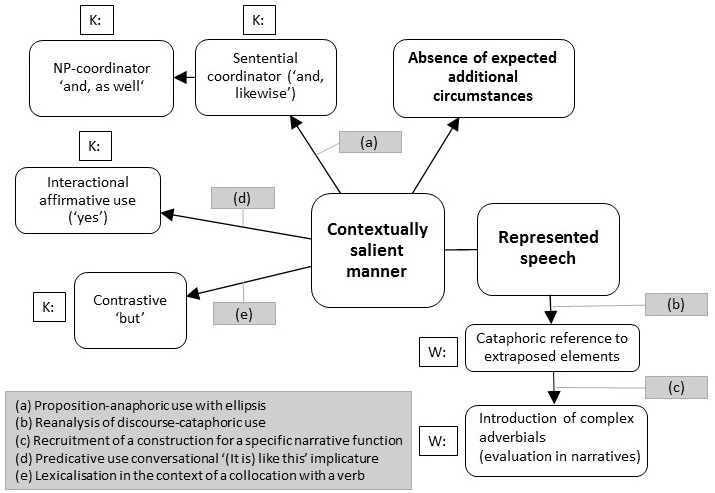
\includegraphics[width=\textwidth]{figures/3_Figure1.jpg}
\label{fig:nikitina:1}
\end{figure}

As syntactic differences determine differences in collocational potential, they are ultimately responsible for the diverse functions the same expression can become associated with, both at the lexical and morphosyntactic levels, and also at the discourse-structure level. Our study discussed examples of all these types of change. The adverbial status of the manner demonstrative in Kambaata is responsible for its frequent use as an argument of the verb ‘become’, causing its combination with the verb to develop into a new lexical expression, the contrastive discourse marker ‘but’. The clause-final position of the manner demonstrative in Wan has enabled it to develop into a syntactic device for introducing extraposed constituents of categories that have no other pronominal equivalents (numerals, adjectives, complex adverbials). At the discourse level, the predicative use of the manner demonstrative in Kambaata has given rise to an interactional affirmative use. In Wan, the extraposition-introducing function of the manner demonstrative has enabled it to introduce complex evaluation-related expressions within traditional narrative discourse. All these uses ultimately depend on the demonstrative’s distributional potential.

Hence, our study has both methodological and theoretical implications. On the methodological side, it shows that comparison of expressions across languages has a lot to gain from paying close attention to the expression’s syntax. When it comes to theory, it serves as a reminder of the need to incorporate fine-grained syntactic information into our models of semantic change. While we tried to make a step in that direction by integrating some constructional information into our semantic map model, further advances should rely on a comprehensive theory of the relationship between syntax and meaning that still needs to be built.

\section*{Acknowledgments}
Affiliation of the authors: CSPC, INALCO CNRS UMR 8135 LLACAN Langage, langues et cultures de l’Afrique. Research for this chapter has been supported by the European Research Council (ERC) under the European Union’s Horizon 2020 research and innovation programme (grant agreement no. 758232).

\section*{Abbreviations}

\subsection*{Wan glosses}

\begin{tabularx}{.45\textwidth}{lQ}
\textsc{adj.foc} & adjunct focus\\
\textsc{aln} & alienable possessor\\
\textsc{cop} & copula\\
\textsc{def} & definite marker\\
\textsc{dimin} & diminutive\\
\textsc{hab} & habitual\\
\textsc{idph} & ideophone\\
\textsc{incl} & inclusive\\
\textsc{intj} & interjection\\
\textsc{log} & logophoric\\
\textsc{nmlz} & nominaliser\\
\textsc{perf} & perfect\\
\end{tabularx}
\begin{tabularx}{.45\textwidth}{lQ}
\textsc{pl} & plural\\
\textsc{pps} & complement-introducing postposition\\
\textsc{prog} & progressive\\
\textsc{prosp} & prospective\\
\textsc{prt} & particle\\
\textsc{quot} & quotative particle\\
\textsc{refl} & reflexive\\
\textsc{rslt} & resultative\\
\textsc{sg} & singular\\
\end{tabularx}


\subsection*{Kambaata glosses}

\begin{tabularx}{.45\textwidth}{lQ}
\textsc{a\_} & adjectival\\
\textsc{abl} & ablative\\
\textsc{acc} & accusative\\
\textsc{add} & additive\\
\textsc{appr} & apprehensive\\
\textsc{asc} & associative\\
\textsc{caus1} & simple causative\\
\textsc{cf} & contrastive focus\\
\textsc{cond} & conditional\\
\textsc{cop1} & existential \textit{yoo-}copula\\
\textsc{cop2} & ascriptive/identificational \textit{\nobreakdash-ha/-ta-}copula\\
\textsc{dat} & dative\\
\textsc{def} & definite\\
\textsc{dem} & demonstrative\\
\textsc{ds} & different subject\\
\textsc{f} & feminine\\
\textsc{gen} & genitive\\
\textsc{ico} & imperfective converb\\
\textsc{icp} & instrumental, comitative, perlative\\
\textsc{intj} & interjection\\
\textsc{ipv} & imperfective\\
\textsc{irr} & irrealis\\
\textsc{m} & masculine\\
\textsc{mid} & middle\\
\textsc{n} & focus-related morpheme\\
\textsc{neg1} & standard negator\\
\end{tabularx}
\begin{tabularx}{.45\textwidth}{lQ}
\textsc{neg4} & converb negator\\
\textsc{neg5} & relative negator\\
\textsc{nmz1} & nominaliser -V\\
\textsc{nmz2} & nominaliser \textit{=bii}\\
\textsc{nmz4} & nominaliser \textit{=r}\\
\textsc{nom} & nominative\\
\textsc{o} & object\\
\textsc{obl} & oblique\\
\textsc{ord} & ordinal\\
\textsc{p\_} & pronominal\\
\textsc{pass} & passive\\
\textsc{pco} & perfective converb\\
\textsc{pfv} & perfective\\
\textsc{poss} & possessive\\
\textsc{prag1} & mitigator \textit{{}-la}\\
\textsc{prag5} & pragmatically determined suffix \textit{{}-be }(function as yet undetermined)\\
\textsc{pred} & predicative\\
\textsc{prf} & perfect\\
\textsc{prog} & progressive\\
\textsc{q} & question\\
\textsc{rel} & relative\\
\textsc{s} & singular\\
\textsc{seq} & sequential\\
\textsc{sg} & singulative\\
\textsc{vv} & vowel lengthening\\
\end{tabularx}

\sloppy\printbibliography[heading=subbibliography,notkeyword=this]
\end{document}
